\documentclass{article}
\usepackage[utf8]{inputenc}
\usepackage[spanish]{babel}
\usepackage{graphicx}
\usepackage{verbatim}
\usepackage{moreverb}
\usepackage{amsmath}
\usepackage{amsfonts}
\usepackage{amssymb}
\usepackage{fancybox}
\usepackage{float}
\usepackage{fancyvrb}
\usepackage{color}
\usepackage{hyperref}
\usepackage{multirow}

\usepackage{anysize}
\marginsize{1cm}{1cm}{0.5cm}{0.5cm}

\renewcommand{\shorthandsspanish}{}

\newcommand{\HRule}{\rule{\linewidth}{0.5mm}}

\begin{document}

\thispagestyle{empty}

%%%%%%%%%%%%%%%%%%%%%%%%%%%%%%%%% PORTADA %%%%%%%%%%%%%%%%%%%%%%%%%%%%%%%%%%%%%%

\begin{titlepage}
\begin{center}

%Espacio antes del logo del itba
\Large \  \\[1.5cm]


\includegraphics[scale=0.40]{Imagenes/logo_itba}\\[1cm]
\textsc{\LARGE Sistemas de inteligencia artificial}\\[1.5cm]
\textsc{\Large Informe preliminar $\text{n}^{\circ}$3}\\[0.5cm]

\HRule \\[0.4cm]
{ \huge \bfseries Red neuronal con aprendizaje supervisado}\\[0.4cm]
\HRule \\[1.5cm]

\Large Autores: \\ [0.25cm]
\begin{tabular}{l @{\ \ -\ \ }l}
\Large Pablo Ballesty & \Large 49359\\[0.2cm]
\Large Nicolás Magni & \Large 48008\\[0.2cm]
\Large Guillermo Liss & \Large 49282 \\[0.2cm]
\end{tabular}



\vspace{1cm}

\vfill
% La fecha queda abajo.
{\large \today}

\end{center}
\end{titlepage}

%%%%%%%%%%%%%%%%%%%%%%%%%%%%%%%%%%%%%%%%%%%%%%%%%%%%%%%%%%%%%%%%%%%%%%%%%%%%%%%%

\begin{abstract}
El objetivo del presente documento es detallar el diseño e implementación de una red neuronal multicapa utilizando aprendizaje supervisado
para resolver las operaciones lógicas de \textit{paridad} y \textit{simetría} para $N$ bits de entrada con $2 \le N \le 5$.
\end{abstract}

\section{Desarrollo}

\subsection{Decisiones de implementación}
A diferencia de la entrega anterior, ahora se crean $N$ redes con $2 \le N \le 5$ para cada método. Luego de entrenar a las redes, los pesos resultantes del aprendizaje quedan persistidos en archivos de texto, que luego se utilizarán para evaluar cada método con la entrada
que ingrese el usuario.
\subsection{Funciones de transferencia}
Se utilizan 2 funciones de transferencia. A continaución se definen las mismas 
\begin{itemize}
 \item \textbf{sigmoid} 
    \begin{equation}
      g(x) = tanh(x)
    \end{equation} 
    \begin{equation}
      g'(x) = 1 - tanh(x)^2
    \end{equation}
  \item \textbf{lineal}
    \begin{equation}
      g(x) = x/4
    \end{equation}
    \begin{equation}
      g'(x) = 1/4
    \end{equation}
\end{itemize}

\subsection{Entrenamiento}
Para entrenar los pesos de las distintas redes, se utiliza \textit{backpropagation} con condición de corte por mínimo error cuadrático aceptable. Al algoritmo de aprendizaje se le realizaron las siguientes mejoras:
\begin{itemize}
 \item \textbf{$\eta$ adaptativo:} Dependiendo de la diferencia entre el error cuadrático de la última época corrida, con el error
cuadrático de la anterior, se realizan pequeños cambios sobre $\eta$. Si esta diferencia es positiva se disminuye el valor de $\eta$ en un porcentaje $b$, y si ocurren
diez diferecias consecutivas negativas se aumenta el valor de $\eta$ en un valor constate $a$. En este caso, $b=0.1$ y $a=0.01$. El fin de estos cambios es que cuando el error aumenta, se realicen cambios pequeños sobre los pesos con el objeto de que el error deje de aumentar, mientras que cuando el error disminuye se busca realizar cambios más grandes con el objetivo de acelerar el aprendizaje.
 \item \textbf{Recomienzo:} el entrenamiento permite fijar una cantidad máxima de épocas a correr, y en caso de no llegar a un error cuadrático menor al esperado, se comienza nuevamente, tomando una nueva inicialización aleatoria. El objetivo de esta  mejora es evitar que el algoritmo se quede siempre en un mínimo local.
\end{itemize}

\section{Resultados}
Para probar el comportamiento del algoritmo de aprendizaje se entrenaron distintas arquitecturas hasta cumplir 
un error cuadrático medio menor a $err=0.01$, para las operaciones lógicas de paridad y simetría, con entradas 
de $N=5$ bits. Se variaron, para la arquitectura de cada operación lógica, el valor $\alpha=$\textit{cantidad de 
neuronas en la capa oculta} y $\eta$ el \textit{learning rate}. \\


Se puede ver en el apéndice, en los cuadros \ref{simetryTable} y \ref{parityTable} para las operaciones lógicas 
de simetría y paridad respectivamente, las comparaciones entre las distintas arquitecturas de redes neuronales.\\

Todos los resultados corresponden a arquitecturas que solo utilizan la función de transferencia \textit{sigmoid}, 
ya que utilizando la función lineal no se logra entrenar a la red. Tampoco se utilizó la función \textit{step}, ya
que por la naturaleza del algoritmo \textit{backpropagation}, ésta no aplica.

\section{Conclusiones}
Se pudo notar que luego de agregar la mejora de $\eta$ adaptativo se logra entrenar a las redes con capa de entrada más grande, ya que sin esta mejora solían caer en mínimos locales. \\
Como se esperaba se lograron entrenar, para las operaciones lógicas de simetría y paridad, redes con arquitecturas a = [N 2 1] y a = [N N 1] respectivamente, siendo $N$ la  cantidad de unidades de entrada, y donde cada elemento $a_i$ es la cantidad de unidades en la capa $i$. \\
Se pudo ver también, la importancia que tiene una buena inicialización de los pesos de la red para lograr entrenarla de forma aceptable, es decir, cumplir el error esperado. Es por esto que en varios casos la mejora de \textit{recomienzo} fue necesaria para alcanzar el objetivo planteado. 


\clearpage
\appendix
\section{Tabla de resultados}
\subsection{Simetría}

\begin{table}[h]
\begin{center}
\begin{tabular}{|r|c|r|}
 \hline
\textbf{$\alpha$} &  \textbf{$\eta$} & \textbf{\# épocas} \\
 \hline
 \multirow{3}{*}{2}
 & 0.5 & 21 \\
 \cline{2-3}
 & 0.25 & 4628 \\
 \cline{2-3}
& 0.1 & $\infty$ \\
 \hline
 \multirow{3}{*}{3}
 & 0.5 & 6072 \\
 \cline{2-3}
 & 0.25 & 2819 \\
 \cline{2-3}
  & 0.1 & 2606 \\
 \hline
 \multirow{3}{*}{4}
  &  0.5 & 42 \\
 \cline{2-3}
  & 0.25 & 190 \\
 \cline{2-3}
  & 0.1 & 149 \\
 \hline
\end{tabular}
\end{center}
\label{simetryTable}
\end{table}


\subsection{Paridad}

\begin{table}[h]
\begin{center}
\begin{tabular}{|r|c|r|}
 \hline
\textbf{$\alpha$} &  \textbf{$\eta$} & \textbf{\# épocas} \\
 \hline
 \multirow{3}{*}{5}
 & 0.5 & 92 \\
 \cline{2-3}
 & 0.25 & 263 \\
 \cline{2-3}
& 0.1 & 206 \\
 \hline
 \multirow{3}{*}{6}
 & 0.5 & 10835 \\
 \cline{2-3}
 & 0.25 & 7686 \\
 \cline{2-3}
  & 0.1 & 3353 \\
 \hline
 \multirow{3}{*}{7}
  &  0.5 & 118 \\
 \cline{2-3}
  & 0.25 & 17011 \\
 \cline{2-3}
  & 0.1 & 3272 \\
 \hline
\end{tabular}
\end{center}
\label{parityTable}
\end{table}

\clearpage

\section{Gráficos}
\subsection{Simetría}

\begin{center}
  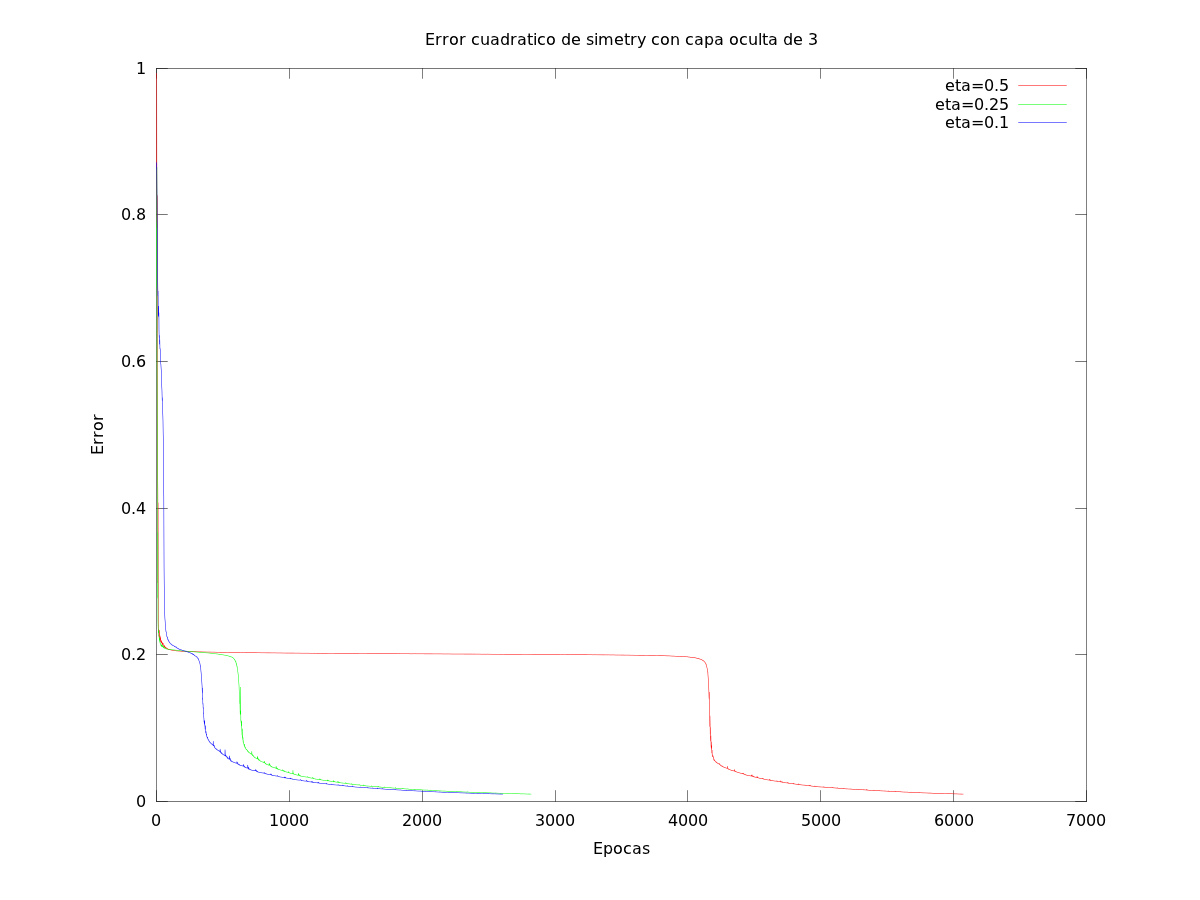
\includegraphics[scale=0.35]{../../doc/results/cuadErrorsimetry_l3.png}
 % cuadErrorsimetry_etaN1_l4.png: 1200x900 pixel, 72dpi, 42.33x31.75 cm, bb=0 0 1200 900

  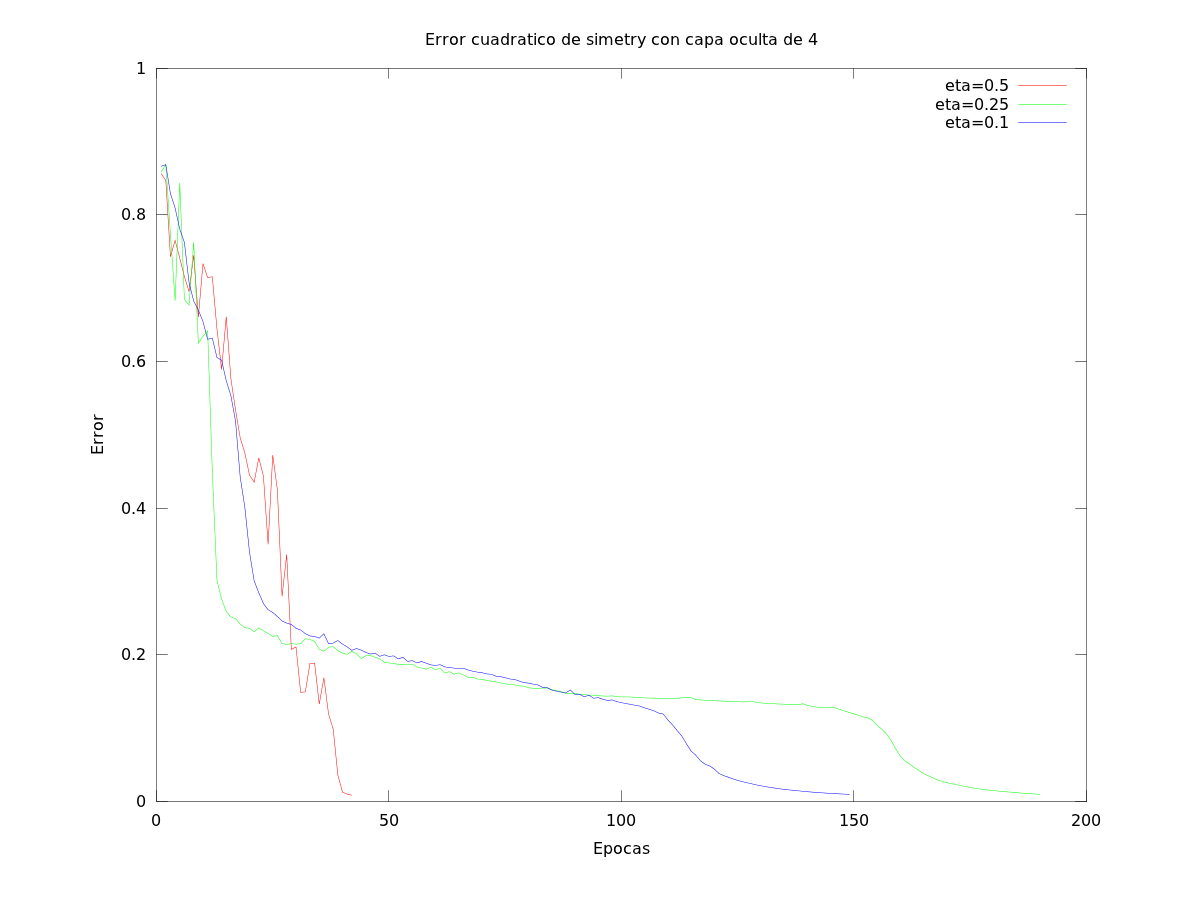
\includegraphics[scale=0.35]{../../doc/results/cuadErrorsimetry_l4.png}
 % cuadErrorsimetry_etaN1_l4.png: 1200x900 pixel, 72dpi, 42.33x31.75 cm, bb=0 0 1200 900
\end{center}

\subsection{Paridad}
\begin{center}
 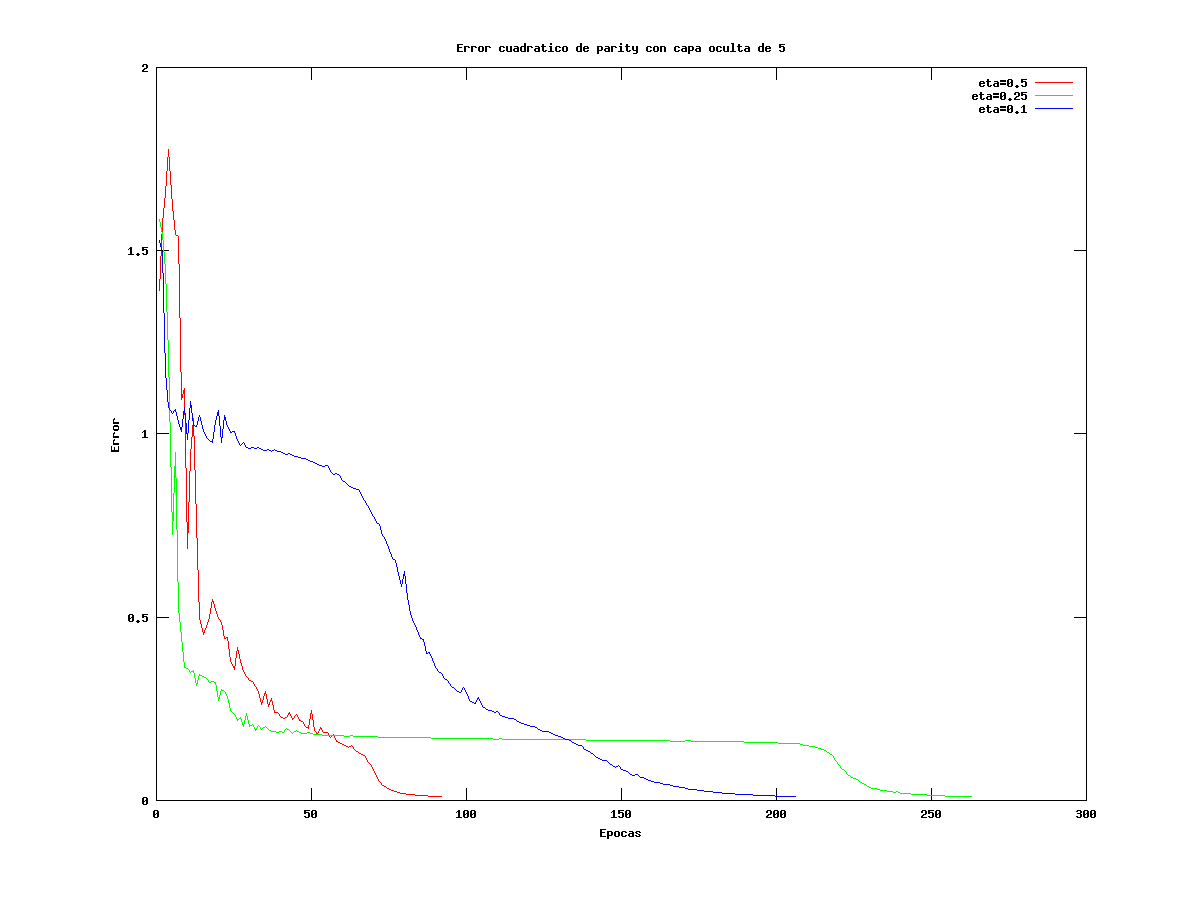
\includegraphics[scale=0.35]{../../doc/results/cuadErrorparity_l5.png}
 % cuadErrorsimetry_etaN1_l4.png: 1200x900 pixel, 72dpi, 42.33x31.75 cm, bb=0 0 1200 900
 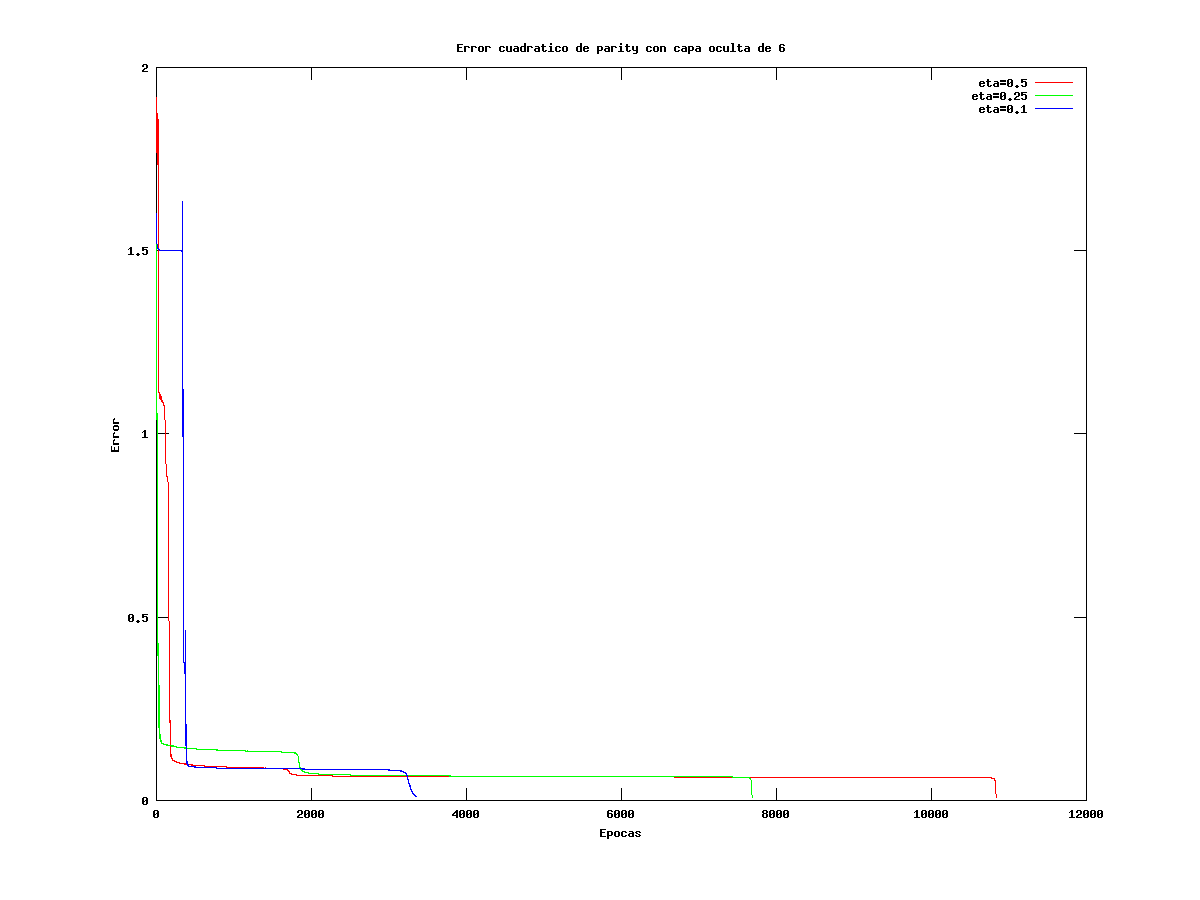
\includegraphics[scale=0.35]{../../doc/results/cuadErrorparity_l6.png}
 % cuadErrorsimetry_etaN1_l4.png: 1200x900 pixel, 72dpi, 42.33x31.75 cm, bb=0 0 1200 900
 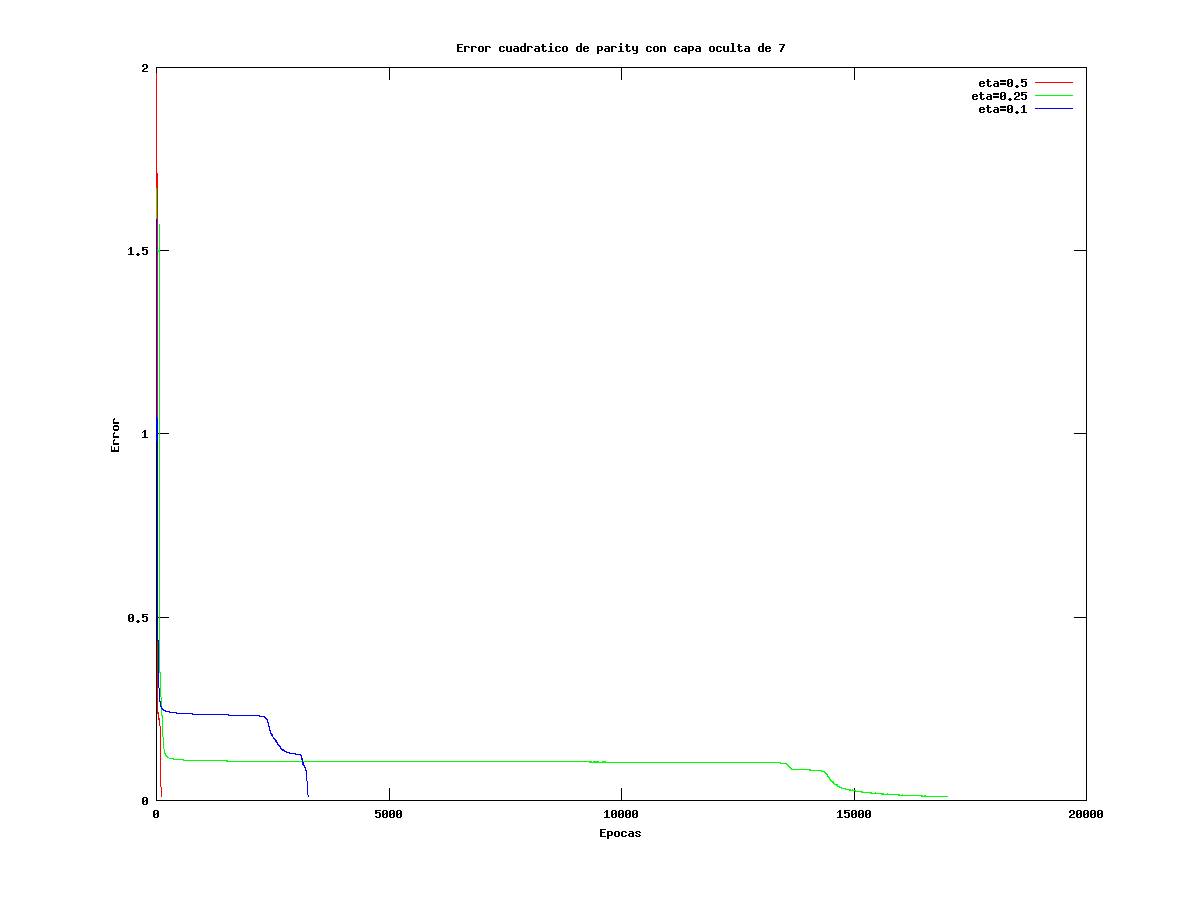
\includegraphics[scale=0.35]{../../doc/results/cuadErrorparity_l7.png}
 % cuadErrorsimetry_etaN1_l4.png: 1200x900 pixel, 72dpi, 42.33x31.75 cm, bb=0 0 1200 900
\end{center}



\end{document}